\documentclass[problem]{mcs}

\begin{pcomments}
  \pcomment{MQ_simple_graphs_short_answer}
  \pcomment{S11.MQ4}
\end{pcomments}

\pkeywords{
   simple_graph
   degree
   handshaking
   handshake
   planar
   face
}


%%%%%%%%%%%%%%%%%%%%%%%%%%%%%%%%%%%%%%%%%%%%%%%%%%%%%%%%%%%%%%%%%%%%%
% Problem starts here
%%%%%%%%%%%%%%%%%%%%%%%%%%%%%%%%%%%%%%%%%%%%%%%%%%%%%%%%%%%%%%%%%%%%%

\begin{problem}
\begin{problemparts}

\problempart A simple graph has 8 vertices and 24 edges.  What is the
average degree per vertex?
\examspace[2.5in]

\begin{solution}
By the Handshaking Lemma, the sum of the degrees of the vertices in
any graph is equal to twice the number of edges.  So in this case, the
sum of the degrees of the vertices is $2\times 24=48$.  With 8
vertices, the average degree per vertex is $\frac{48}{8}=6$.
\end{solution}

\problempart A connected planar simple graph has 5 more edges than it
has vertices.  How many faces does it have?

\examspace[2.5in]

\begin{solution}
Denoting the number of vertices by $v$, the number of edges by $e$,
and the number of faces by $f$, Euler's Formula states that $v-e+f=2$.
But here, $e=v+5$.  Substituting gives $v-(v+5)+f=2$ and hence $f=7$.
\end{solution}

\problempart\label{1morevertex}
A connected simple graph has one more vertex than it has
edges.  Explain why it is a planar graph.

\examspace[2in]

\begin{solution}
Let $G$ denote any such graph.  Now, any graph with $v$ vertices but
fewer than $v-1$ edges cannot possibly be connected.  So every edge in
$G$ is a cut edge, and therefore $G$ is acyclic.  So $G$ is a tree and
must be planar.
\end{solution}

\examspace

\problempart How many faces does a planar graph from
part~\ref{1morevertex} have?

\examspace[2in]

\begin{solution}
Since the graph is connected and acyclic, it only has one face.
\end{solution}


\problempart How many distinct isomorphisms are there between the
graph given in Figure~\ref{fig:self_isomorphism} and itself?  (Include
the identity isomorphism.)

\begin{figure}[h]
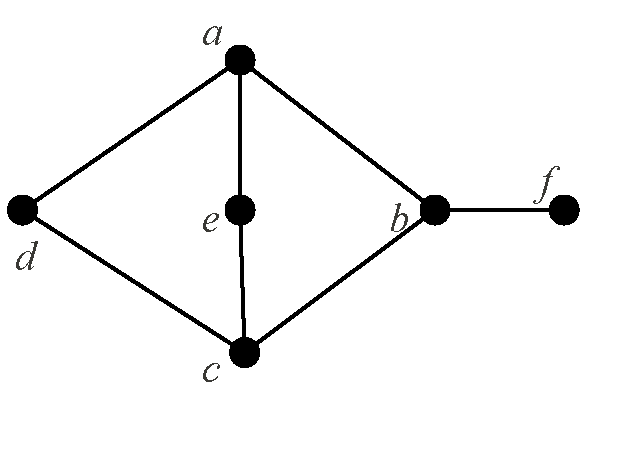
\includegraphics[width = 2in]{MQ_self_isomorphism}
\caption{\label{fig:self_isomorphism}}
\end{figure}

\begin{solution}
Only vertex $f$ has degree 1, so in any self-isomorphism, $f$ must map
to itself.  $b$ is the only vertex to be adjacent to a degree-1
vertex, so $b$ must also map to itself.  $a$ and $c$ are both degree-3
vertices, and $d$ and $e$ are both degree-2 vertices.  It is clear
from examining the graph that $a$ can be mapped to $c$ and $c$ to $a$,
or each of $a$ and $c$ can be mapped to itself.  Independently, and
similarly, $d$ can be mapped to $e$ and $e$ to $d$, or each of $d$ and
$e$ can be mapped to itself.  The only possible isomorphisms, then,
are obtained by choosing one of the two possible mappings for $a$ and
$c$ and, independently, one of the two possible mappings for $d$ and
$e$.  The result is $2\times2=4$ possible isomorphisms.
\end{solution}

\end{problemparts}
\end{problem}

\endinput
